%%% alternativ: english, ngerman
\documentclass[ngerman,
 paper=a4, 11pt,  twoside, openright, BCOR=7mm, DIV12, headinclude=false, listof=totoc, index=totoc,bibliography=totoc,headinclude=false,chapterprefix=on]{scrreprt}

% Einseitige Variante:
%\documentclass[ngerman, paper=a4, 11pt, cleardoubleempty, fancyheaders, oneside, openright, BCOR=7mm, DIV12, listof=totoc, index=totoc,bibliography=totoc, headinclude=false]{scrreprt}


%Falls man Biber anstatt bibtex verwendet und nicht die Makefile nutzt, die nächste Zeile auskommentieren
%\def\usebusybiber{1}

\usepackage[
fancyheaders %hübsche Kapitelüberschriften
]{fb10-format}


%%%%%%%%%%%%%%%%%%%%%%%%%%%
%% Daten für Deckblatt und eid. Erklärung
%%%%%%%%%%%%%%%%%%%%%%%%%%%
\title{Implementation of a LaTeX Style for Diploma, Bachelor, and Master Theses}
\author{Erika Dürstefrau}
\matrikelno{123456}
\thesis{Diplömchenarbeit}
\profName{Prof. Dr. Trestermind}
\assistentName{MSc. Mini Humpen}
\date{02. Februar 2222}
%\aglogo{./graphics/cs_logo_nl_blue.pdf}
%\aglogo{./graphics/comsys_logo.pdf}
\institutName{Institut für Brauereiwesen}
\arbeitsgruppenName{Arbeitsgruppe Topologische Gläser}



\automark[section]{chapter}
%Neue Mathematische Operationen definieren
\DeclareMathOperator{\dom}{dom}
%Latex bei Worttrennung helfen
\hyphenation{Staats-ver-trag Stau-be-cken ge-sam-melt}
%Theorem, Satz..
\newtheorem{theorem}{Theorem}
\newtheorem{definition}{Definition}
\newtheorem{satz}{Satz}

\begin{document}
	%===================================	
	% Deaktiviere "a für ä, wir nutzen eh UTF8
	%===================================	
	\iflanguage{ngerman}{
	\shorthandoff{"}}
	%===================================	
	%Druck die Todo-Liste
	%===================================
	\listoftodos

	%===================================
	% Titlepage
	%===================================
	\pagenumbering{roman}

	% Titelblatt
	\maketitle
	\cleardoublepage
	
	%===================================
	% Erzeuge divere Listen (Tabelle,Quellcode)
	%===================================
	\input{text/abstract}
	\cleardoublepage
	
	\tableofcontents
	\listoffigures
	\listoftables
	\lstlistoflistings	
	\printglossary[type=acronym]
	\printglossary

    \cleardoublepage
    \pagenumbering{arabic}
	\StartMainpart %Fuer die Fancy-Headers
	%===================================
	% Die eigentliche Arbeit
	%===================================	
    \chapter{The FB10 Template}
Auch hier sollte ein Text stehen. Jedes Kapitel braucht ein paar einleitende Sätze. Niemals beginnt ein Kapitel mit einem neuen Abschnitt (\textit{Sektion})!
\section{Anleitung zum Template}
\label{secHowTo}
%==============================================================================
Für die  Benutzung des \gls{FB10}-Templates gibt es einige wichtige Regeln:
\begin{enumerate}
    \item Benutze \gls{pdflatex} oder \texttt{latexmk} zum kompilieren des  Latex Quellcodes. Für Linux liegt eine Makefile bei.

	\item Wir versuchen immer Vektorgrafiken zu verwenden (\texttt{svg}, \texttt{ai}, \texttt{pdf}) und vermeiden gerasterte Grafiken (\texttt{jpg}, \texttt{png}, \texttt{tiff}, \texttt{gif}, \texttt{bmp}). Als Programme bieten sich dabei \href{http://www.inkscape.org/}{Inkscape} (OpenSource), Adobe Illustrator (z.B. auf dem IVV5-Terminalserver) oder CorelDraw (Gibt es beim ZIV) an. 
	\item Bevor du das aussehen dieses Templates veränderst, sprich mit deinem Betreuer
	\item Füge gelesenen Paper und ähnliche in die \texttt{bibliography.bib} ein; Benutze dabei \href{http://jabref.sourceforge.net/}{JabRef} als Editor.
	\item Floating Umgebungen (Tabellen, Abbildungen, etc) machen sich oft oben auf der Seite ganz gut.
	\item Jede Floating-Umgebung hat immer eine kurze, als auf eine lange Beschreibung! 
	\item Quellcode sollte in einer Extra-Datei gespeichert werden und mittels entsprechenden Befehl in das Dokument eingebunden werden. Sehr kurze Abschnitte kann man auch direkt in die Tex-File schreiben.
	\item In einer Abschlussarbeit findet sich in der Regel nicht sehr viel Quellcode....
\end{enumerate}

\section{\LaTeX Examples}

Zu den folgenden Elementen finden sich Beispiele in dieser Vorlage
\begin{itemize}
    \item Aufzählungen, also das hier
	\item Aufzählungen auf Seite \pageref{example:enumeration}
	\item Beschreibungen auf Seite \pageref{example:description}
	\item Tabellen auf Seite \pageref{tab:table}
	\item Quellcode auf Seite \pageref{lst:useless}
	\item abgesetzte Mathematische Formeln Seite \pageref{eqn:formula}
	\item Quellenverweise Seite \pageref{example:reference}
	\item Acronyme, siehe das Paket \texttt{glossaries} 
	\item Glossar, siehe die Datei \texttt{glossary.tex}
	\item Bytefelder, siehe Seite \pageref{fig:bytefield}
	\item Referenzierung von Abschnitten, Abbildungen, Quellcode, Tabellen und vielen anderen Sachen finden sich im gesamten Dokument
	\item Abbildung auf Seite \pageref{fig:smiley}
	\item Theoreme, Satz, Beweis, Definition, inklusive einer Umgebung für Formeln die über mehrere Zeilen gehen auf Seite \pageref{example:theorem.multiline}
	\item Mathematische Diagramme auf Seite \pageref{example:diagram}
	\item Unterabbildungen auf Seite \pageref{fig:meth:bgsub:whole}
	\item Den Mathemodus innerhalb einer Zeile, z.B. $\exists x \in \{1,\frac{3}{2},2,\ldots,9\}$
	\item Anmerkungen mittels des Todo-Paketes \pageref{example:todo} und auch für fehlende Bilder \pageref{fig:meth:bgsub:whole}
\end{itemize}

Zur Verwendung des Glossars muss der Befehl \texttt{makeindex} wie folgt benutzt werden:
\begin{verbatim}
makeindex -s main.ist -t main.glg -o main.gls main.glo
\end{verbatim}
Für die Liste der Akronyme
\begin{verbatim}
makeindex -s main.ist -t main.alg -o main.acr main.acn
\end{verbatim}
Unter Linux kann auch die MakeFile benutzt werden. Dazu einfach auf der Konsole im jeweiligen Ordner \texttt{make} eingeben. 
Alle temporären Dateien lassen sich mit \texttt{make clean} löschen.

\newpage
\section{Weitere Dokumentation}
Wir haben auf unserer Homepage einige praktische Dokumente für die Arbeit mit Latex gesammelt, siehe \href{http://www.uni-muenster.de/Comsys/en/teaching/technical_writing.html}{hier}.
Latex-Pakete und deren Doumentation finden sich in der Regel im \href{http://www.ctan.org/}{Comprehensive TeX Archive Network}.

Einige Links zu den wichtigsten Paketen:
\begin{itemize}
	\item \href{http://tug.ctan.org/cgi-bin/ctanPackageInformation.py?id=bytefield}{bytefield - Create illustrations for network protocol specifications}
	\item \href{http://tug.ctan.org/cgi-bin/ctanPackageInformation.py?id=colortbl}{colortbl - Add colour to LaTeX tables}
	\item \href{http://tug.ctan.org/cgi-bin/ctanPackageInformation.py?id=eqnarray}{eqnarray - More generalised equation arrays with numbering}
	\item \href{http://tug.ctan.org/cgi-bin/ctanPackageInformation.py?id=glossaries}{glossaries - Create glossaries and lists of acronyms}
	\item \href{http://tug.ctan.org/cgi-bin/ctanPackageInformation.py?id=graphicx}{graphicx - Enhanced support for graphics}
	\item \href{http://tug.ctan.org/cgi-bin/ctanPackageInformation.py?id=listings}{listings - Typeset source code listings using LaTeX}
	\item \href{http://tug.ctan.org/cgi-bin/ctanPackageInformation.py?id=pdflscape}{pdflscape - Make landscape pages display as landscape}
	\item \href{http://tug.ctan.org/cgi-bin/ctanPackageInformation.py?id=supertabular}{supertabular - A multi-page tables package}
	\item \href{http://tug.ctan.org/cgi-bin/ctanPackageInformation.py?id=xcolor}{xcolor - Driver-independent color extensions for LaTeX and pdfLaTeX}
\end{itemize}
 %%% read this!!!
	\chapter{Introduction} 

\label{cha:introduction}
%==============================================================================

%\blindtext

%\section{Motivation}
\label{sec:motivation}
%==============================================================================

\blindtext \cite{Loepmeier:2015TR} \label{example:reference}

%http://get-software.net/macros/latex/contrib/caption/subcaption.pdf
\begin{figure}	
	\centering
	\begin{subfigure}[t]{0.45\textwidth}
		\caption{Logo des Institut für Informatik}
		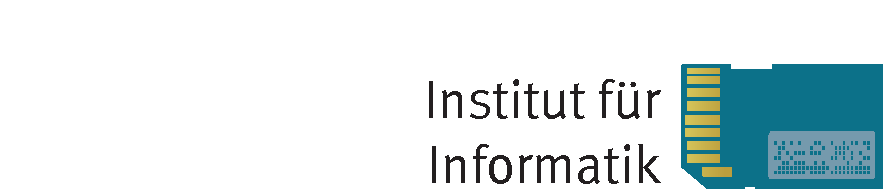
\includegraphics[width=1.0\textwidth]{graphics/cs_logo_nl_blue.pdf}
	\end{subfigure}
	\begin{subfigure}[t]{0.45\textwidth}
		\caption{Logo der Uni}
		
\includegraphics[width=1.0\textwidth]{graphics/wwu-logo-neu.pdf}
	\end{subfigure}

	\begin{subfigure}[t]{0.45\textwidth}		
		\phantomsubcaption\label{fig:inner}
		\missingfigure[figwidth=\textwidth]{Logo des FB10}
	\end{subfigure}
	\begin{subfigure}[t]{0.45\textwidth}
		\phantomsubcaption
		\missingfigure[figwidth=\textwidth]{Logo der Numerik}		
	\end{subfigure}
\caption[Logos der Uni]{Logos der Uni. Dabei kann man auch wieder referenzieren wie auf \subref{fig:inner}. Dabei muss noch nicht einmal eine Unterüberschrift existieren. Dies ist besonders praktisch, falls die Buchstaben schon in den Bildern vorhanden sind. Details \href{http://get-software.net/macros/latex/contrib/caption/subcaption.pdf}{hier}
}
\label{fig:meth:bgsub:whole}
\end{figure}
%
%\Blindtext
%
%\section{Thesis Structure}
%\label{secStruktur}
%%==============================================================================
%
%\Blindtext

    \section{Related Work}
\label{sec:related_work}
%==============================================================================
\Blindtext


\begin{figure}[t]
	\centering
	\fbox{\includegraphics[width=4cm]{./graphics/smiley}}
	\caption[This is a smiley]{This is a smiley; it has no particular use but looks nice. \blindtext}
	\label{fig:smiley}
\end{figure}

\begin{figure}[t]
	\centering
	\fbox{\includegraphics[width=4cm]{./graphics/smiley}}
	\caption[This is a smiley 2]{This is a smiley 2; it has no particular use but looks nice.}
	\label{fig:smiley2}
\end{figure}

\Blindtext


\begin{description} \label{example:description}
	\item[Lorem:] Nam liber tempor cum soluta nobis eleifend option congue nihil 
	\item[Ipsum:] Duis autem vel eum iriure dolor in hendrerit in vulputate velit esse molestie consequat
	\item[Dolor:] At vero eos et accusam et justo duo dolores et ea rebum
\end{description}


\Blindtext

    \chapter{Thesis Contribution} 
\label{cha:thesis_contribution}
%==============================================================================
\blindtext
\section{Implementation}
\label{sec:implementation}
%==============================================================================
\Blindtext

\begin{figure}[t]
    \centering
    \begin{bytefield}{32}
        \bitheader{0-31}\\
        \begin{rightwordgroup}{Header}
            \bitbox{16}{Source}\bitbox{16}{Destination}\\
            \wordbox{1}{Acknowledgement}\\
            \wordbox{1}{Sequencenumber}
        \end{rightwordgroup} \\
        \wordbox[lrt]{1}{Data} \\
        \skippedwords \\
        \wordbox[lrb]{1}{} \\
    \end{bytefield}
    \caption[Packet Format]{Packet Format of the protocol specified in this section}
    \label{fig:bytefield}
\end{figure}
\Blindtext

%%% listings with same name share a linecounter %%%
%%% include source code from external file: \lstinputlisting[<Options>]{path/file.php} %%%
\begin{lstlisting}[caption=Useless code,label=lst:useless, name=useless, language=C++]
int main(int argc, char** argv) {
    int i;
    //Kommentar
    for(i=0; i<10; i++) { %*\label{lstref:loop}%*
        printf("I will graduate!\n");
    }
    return 0;
}
\end{lstlisting}
\Blindtext
\label{example:todo}
\todo{was heisst das hier eigentlich?}
\Blindtext
    \section{Experiments}
\label{sec:experiments}
%==============================================================================
\Blindtext
\begin{enumerate} \label{example:enumeration}
	\item At accusam
	\item aliquyam diam
	\item diam dolore
\end{enumerate}

\Blindtext
    \chapter{Thesis Outcome}
\label{cha:thesis_outcome}
%==============================================================================
\blindtext
\section{Evaluation}
\label{sec:evaluation}
%==============================================================================
\Blindtext
\begin{eqnarray} \label{eqn:formula}
    Prob(W_A < W_B) &=& \frac{1}{2} * \frac{3}{4} + \frac{1}{2} * \frac{2}{4} = \frac{5}{8} = 0.625 \\
    Prob(W_A < W_B) &=& \frac{1}{2} * \frac{7}{8} + \frac{1}{2} * \frac{6}{8} = \frac{13}{16} = 0.8125
\end{eqnarray}
\Blindtext

\begin{table}
    \centering
    \begin{tabular}{l|c|p{5cm}} \toprule
        A & B & C \\ \midrule
        1 & Ut wisi enim & nostrud exerci tation ullamcorper suscipit lobortis nisl ut aliquip ex ea commodo consequat. Duis autem vel eum \\
        2 & Ut wisi enim & nostrud exerci tation ullamcorper suscipit lobortis nisl ut aliquip ex ea commodo consequat. Duis autem vel eum \\
        3 & Ut wisi enim & nostrud exerci tation ullamcorper suscipit lobortis nisl ut aliquip ex ea commodo consequat. Duis autem vel eum \\
        \bottomrule
    \end{tabular}
    \caption[Useless Table]{Useless Table in a floating environment; the rightmost column is a 5cm wide paragraph; paragraphs do break lines}
    \label{tab:table}
\end{table}

    \section{Conclusion}
\label{sec:conclusion}
%==============================================================================
\blindtext



\begin{theorem}[Lorenz-Langmann]
Dieses Theorem hat eine witzige Vermutung, die hier nicht näher ausgeführt werden soll.
Es folgt der Beweis mit einem Beispiel für die mehrzeilige IEEE Equationarray Umgebung:
\begin{IEEEproof}[Beweis]\label{example:theorem.multiline}
Der Beweis ist sehr simpel. Und er eigentlich ist es auch keiner.
\begin{IEEEeqnarray}{rCl}
a	& = 	& b + c				\\
	& = 	& d + e + f + g + h
	+ i + j + k \nonumber		\\
	&		& +\> l + m + n + o		\\
	\noalign{Mittels des \texttt{noalign}-Befehlt lässt sich leicht ein Text innerhalb der IEEEeqnarray-Umgebung einfügen}
	& = 	& p + q + r + s
\end{IEEEeqnarray}
\end{IEEEproof}
\end{theorem}

\begin{definition}[$\mathfrak{t}$-Funktion]
Die Funktion $\mathfrak{t}_W:\mathbb{R}\rightarrow W$ ist definiert durch:
\[
\mathfrak{t}_W(x):=\max\left\lbrace k \in W \right\rbrace
\]
Macht keinen großen Sinn, oder?
\end{definition}

\Blindtext
\todo{Das steht total losgelöst vom Text, bitte ändern!}
 Es folgt ein tolles Diagramm:
 \label{example:diagram}
\[
\begin{tikzcd}[column sep=huge]
\mbox{} & A \arrow{r}{f} \arrow{d}{a} & B \arrow{r}{g} \arrow{d}{b} & C \arrow{r} \arrow{d}{c} & 0 \\
0 \arrow{r} & A' \arrow{r}{f'} & B' \arrow{r}{g'} & C' \end{tikzcd} \]
\Blindtext


	%Literaturverzeichnis
	\appendix		
	\ifdefined\usebusybiber

		\printbibliography 
	\else
		\bibliographystyle{unsrt}
		\bibliography{bibliography}
	\fi
	%Anhang
    \chapter{For Example: Sourcecode}
\lstinputlisting[
	language=C++
	%, title=Falls nicht der Dateinamen als Titel stehen soll.	 
]{src/example.c}

\chapter{Second one}
\blindtext    
    
    %===================================
    % Offizieller Teil
    %===================================
    \cleardoublepage
    \pagestyle{empty}
   	\affirmation
\end{document}
